\documentclass{article}
\usepackage{tikz}
\usetikzlibrary{arrows.meta}

\begin{document}

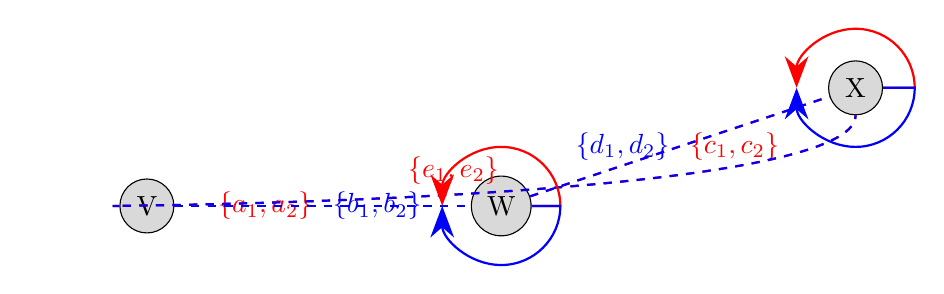
\begin{tikzpicture}[scale=1.5]
    % Nodes
    \node[circle, draw, fill=gray!30] (V) at (0,0) {V};
    \node[circle, draw, fill=gray!30] (W) at (3,0) {W};
    \node[circle, draw, fill=gray!30] (X) at (6,1) {X};

    % Edges
    \draw[red, dashed, thick] (V) -- node[left] {$\{a_1, a_2\}$} (W);
    \draw[blue, dashed, thick] (V) -- node[right] {$\{b_1, b_2\}$} (W);
    \draw[red, dashed, thick] (W) -- node[right] {$\{c_1, c_2\}$} (X);
    \draw[blue, dashed, thick] (W) -- node[left] {$\{d_1, d_2\}$} (X);
    \draw[red, dashed, thick] (V) .. controls +(180:1) and +(-90:1) .. node[above] {$\{e_1, e_2\}$} (X);
    \draw[blue, dashed, thick] (V) .. controls +(180:1) and +(-90:1) .. node[above] {} (X);

    % Arrows
    \draw[red, thick, -{Stealth[length=4mm]}] (W) -- ++(0:.5) arc (0:180:.5);
    \draw[blue, thick, -{Stealth[length=4mm]}] (W) -- ++(0:.5) arc (0:-180:.5);
    \draw[red, thick, -{Stealth[length=4mm]}] (X) -- ++(0:.5) arc (0:180:.5);
    \draw[blue, thick, -{Stealth[length=4mm]}] (X) -- ++(0:.5) arc (0:-180:.5);
\end{tikzpicture}

\end{document}